\documentclass[10pt]{report}
\usepackage{a4wide}
\usepackage{amsmath}
\usepackage{amsfonts}
\usepackage{amssymb}
\usepackage{amsthm}
\usepackage{longtable}
\usepackage{graphicx}

\begin{document}
\newcommand{\doctitle}{Proposal}
\begin{titlepage}
	\begin{center}
		~\\
		\vspace{100pt}
		\Huge{Additional Component CG 2008-2009}\\
		\vspace{50pt}
		\huge
		``block editor: geometric modeling''\\
		\doctitle\\
		\vspace{100pt}
		\large
		Eindhoven University of Technology\\
		Computer Science and Engineering master\\
		\vspace{50pt}
		\begin{tabular}{ll}
			Bart van Arnhem & 0557184 \\
			Maarten Manders & 0573419 \\
		\end{tabular}\\
		\vspace{50pt}
		\today
	\end{center}
\end{titlepage}

\tableofcontents

%
% Chapter Introduction
%
\chapter{Introduction}
This is the first document that has to be delivered for the ``additional component CG 2008-2009''(2IV05) course lectured at the TU/e. The document proposes our solution to a chosen assignment. The assignment for which we propose is ``block editor: geometric modeling''.\\

This document describes the intended solution to the problem described in the assignment. The description consists of functional, interactive and presentational specifications, a description of the used development environment and a brief planning scheme.

%
% Chapter Description
%
\chapter{Description}
This chapter describes the wat kind of software that will be developed. Also, the chosen programming language and environment are mentioned.

\section{Software description}
We like to develop a geometric model editor which is based on the combination of simple geometric objects. The ultimate goal is that users compose objects which they can use to create more complex objects. In order to create simple objecs a small set of basic objects, such as spheres, piramides, cubes, etc will be added.\\

Users create objects using two actions: adding and removing of objects. Users can build the basic shape of an object by adding objects to each other, they can create more detailed shapes by removing specific object shaped parts from a created object.\\

Because there will only be a small number of standard objects will be specified, users can create more complex objects which they can use to create even more complex objects. This stepwise creation process leads to a quick and easy way to create very complex shapes.

\section{Programming language and environment}
Our software will be developed using the Java programming language in combination with OpenGL. During the literature study phase (see chapter \ref{chap:planning}) the OpenGL library that will be used will be determined.

%
% Chapter Specification
%
\chapter{Specification}
This chapter is divided in two sections, which all specify different aspects of our system. The ``Functionality'' section describes the functionality of our software. The ``Interaction and presentation'' section describes the ways how the users of our software can interact with the software.

\section{Functionality}
\label{sect:functionality}
This section describes the functionality of the software. There are two kinds of functionality that will be added. ``Core functionality'' is that part of the software that must be implemented in order to make it work properly. ''Extra functionality'' is that part of the software that makes it more appealing. If time permits, all the functionality will be implemented, otherwise parts of the extra functionality will be dropped.\\

\noindent The core functionality consists of: \\
\vspace{-10pt}
\begin{enumerate}
	\item Object editing window
	\item Object selector window
	\item Shape loading
	\item Shape saving
	\item Shape intersection
	\item Shape difference
	\item Zooming
	\item Rotation
	\item Wire frame view
\end{enumerate}
\bigskip
\noindent The extra functionality consists of: \\
\vspace{-10pt}
\begin{enumerate}
	\item Solid view
	\item Texturing
	\item Adding temporary shapes
	\item Preview
	\item Lighting
\end{enumerate}

\subsection{Possible extra functionality (if there is time)}
Possibility to specify a ``weight'', meaning only a certain amount of material is added or removed from the geometric object.

\section{Interaction and presentation}

\begin{figure}[h]
\centering
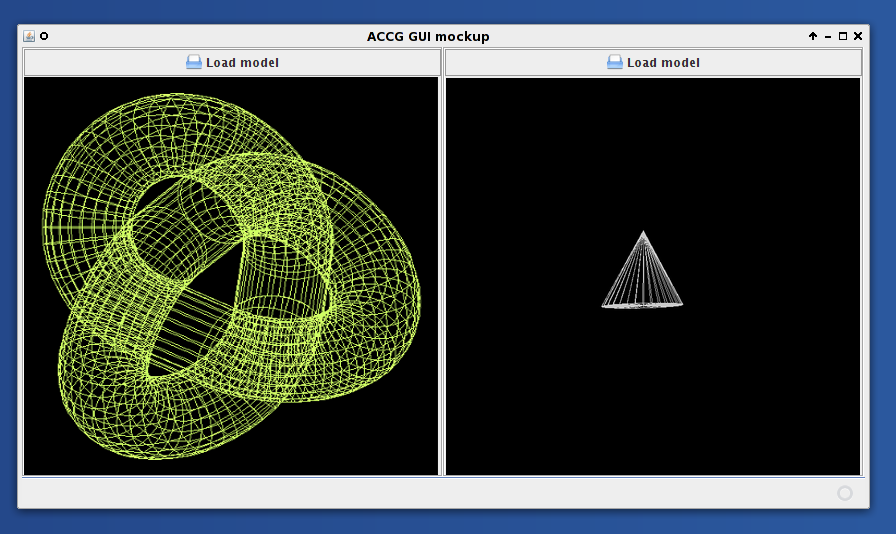
\includegraphics[width = 0.8\textwidth]{../resources/gui_mockup/1}
\caption{\emph{Mockup of the graphical user interface}} \label{gui_mockup}
\end{figure}

Figure \ref{gui_mockup} displays a mockup of the graphical user interface. The right and left frame contain respectively the ``building block'' and the ``result'' models. Using the mouse both models can be zoomed an rotated in an intuitive way (like in 3D Studio Max).\\

Clicking with the left mouse button in the left frame will result in the model loaded in the right frame being added to the result model at the clicked position. Using the right mouse button the model can be removed from the result model. \\

Both models can be loaded from a file using the ``Load model'' buttons. The result model can also be saved to a file. \\

To give the user an idea of where the material is going to be added or removed a semi transparent version of the ``building block'' model is rendered at the mouse cursor. \\

%
% Chapter Planning
%
\chapter{Planning}\label{chap:planning}
This chapter contains three sections. The section ``Tasks'' offers an overview of the tasks that have to be performed in order to complete our software. The section ``Deadlines'' shows an overview of these tasks and their corresponding deadlines. In the last section, ``Possible resources'', several sources witch we can study are listed.

\section{Tasks}
This section describes the tasks that have to be performed in order to complete our software. Every task is composed of a short title and a description. In the next section the tasks described in this section will be mapped to deadlines.\\

\begin{enumerate}
	\item \textbf{Architecture:}\\
		Here the components of which our software consists are defined.
	\item \textbf{Literature study:}\\
		Research to find usable algorithms to intersect and differentiate shapes, etc.
	\item \textbf{Environment:}\\
		Find and install libraries required for the development of the software.
	\item \textbf{Java project and GUI:}\\
		Create a java project and the GUI for the software.
	\item \textbf{Demo (midterm deadline I):}\\
		A small demo and presentation of the GUI and architecture of the software and the algorithms that will be used.
	\item \textbf{Model loading and saving:}\\
		Implementation of the modeling part of the software. Including loading and saving of objects.
	\item \textbf{Transformation and basic model manipulation:}\\
		Implementation of the basic actions that can be performed on models.
	\item \textbf{Demo (midterm deadline II):}\\
		A small demo and presentation of the basic actions that can be preformed on models.
	\item \textbf{Extra functionality:}\\
		Implementation of the extra actions that can be preformed on models.
	\item \textbf{Demo and report:}\\
		The final demo and the end report of our software.
\end{enumerate}

\section{Deadlines}
This section maps the tasks described in the previous section to corresponding deadlines, also a time estimate (in hours per group member) for each separate task is specified.\\

\begin{longtable}{|p{2pt} l|l|l|}
	\hline
	\textbf{Task}    &                                   & \textbf{Deadline}  & \textbf{Time}\\
	\hline
	1. & Architecture                                   & Sunday 07/09/2008  & 4 \\
	2. & Literature study                               & Sunday 14/09/2008  & 8 \\
	3. & Environment                                    & Sunday 21/09/2008  & 4 \\
	4. & Java project and GUI                           & Sunday 12/10/2008  & 12 \\
	5. & \textbf{Demo (midterm deadline I)}             & Tuesday 14/10/2008 & 4 \\
	6. & Model loading and saving                       & Tuesday 04/11/2008 & 32 \\
	7. & Transformation and basic model manipulation    & Sunday 23/11/2008  & 32 \\
	8. & \textbf{Demo (midterm deadline II)}            & Tuesday 25/11/2008 & 4 \\
	9. & Extra functionality                            & Sunday ??/01/2009  & 6 \\
	10.& \textbf{Demo and report (submission deadline)} & Sunday ??/01/2009  & 34 \\
	\hline
	& \textbf{Total}                                    &                    & \textbf{140} \\
	\hline
\end{longtable}

\section{Possible resources}
\begin{enumerate}
	\item http://www.win.tue.nl/$\sim$wstahw/2IV40/2-implicits-2007-2008.pdf\\
          section on blending (pages 15-17).
\end{enumerate}

\end{document} 